\section{RationalGRL: Logical Framework}
\label{sect:formalframework}

In Section~\ref{sect:overview}, we have shown through a language definition and informal examples from our case study that it is possible to trace elements of the goal model back to their underlying arguments (\textbf{requirement 2}), and that it is possible to determine the effect of changes in the underlying argumentation on the goal model, and vice versa (\textbf{requirement 3}). A formal rendition of this traceability will be presented in this section, in which we present a logical formalization of RationalGRL. This is done for multiple reasons: (i) Most approaches in formal argumentation (cf. Section~\ref{sect:background:pras}) use formal logic, allowing us to employ existing technique directly in order to compute which arguments are accepted and which are rejected, (ii) we can be more precise about how critical questions are answered, (iii) we can show that RationalGRL models can be translated to valid GRL models and vice versa in a precise way, and (iv) the formal approach is a basis for automating the framework in terms of tool support, which we present in the next section.

In Sections \ref{sect:formalframework:grl} and \ref{sect:formalframework:rationalgrl} we formalize a static representation of our framework based on the metamodel (Figure~\ref{fig:metamodel}). We first provide a formal specification of a GRL model in Section~\ref{sect:formalframework:grl}, and we extend this with arguments and attack links in the Section~\ref{sect:formalframework:rationalgrl}, hereby obtaining a formal specification of a RationalGRL model. In Section~\ref{sect:formalframework:translation} we then present algorithms in order to translate a GRL model into a RationalGRL model, and vice versa. Finally, in Section~\ref{sect:algorithms} we develop algorithms for instantiating argument schemes and answering critical questions and thus formally capture the \textsf{INTRO}, \textsf{REPLACE} and \textsf{DISABLE} operations of which examples were previously given in Section~\ref{sect:overview:examples}. 

\subsection{Formal Specification of GRL}
\label{sect:formalframework:grl}

We formalize a GRL model based on the metamodel (Figure~\ref{fig:metamodel}), starting with intentional elements and actors.

Throughout this section, we adopt the convention that variables start with a lowercase letter (e.g, $id$, $i$, $j$, $name$, $goal$), and sets and constants start with an uppercase letter (e.g., $Type, AND, Goal$). We begin by defining general elements of our language that we use in subsequent definitions.

\begin{definition}[General definitions]
\label{def:set-definitions}
We define the following sets:
\begin{itemize}
\item $IETypes = \{Softgoal, Goal, Task, Resource\}$,
\item $LinkTypes = \{PosContr, NegContr, Dep, Decomp\}$\footnote{Recall from Section~\ref{sect:background} that for contribution links we only distinguish between positive and negative contributions. Extending the formalization model to include all the GRL values is straightforward but has been omitted here for conciseness.},
\item $Types = IETypes \cup LinkTypes\cup\{Actor, ActIE, GenArg\}$,
\item $Names$ is a finite set of strings,
\item $DecompTypes = \{AND,OR,XOR\}$.
\end{itemize}
\end{definition}
Next, we define an intentional element.

\begin{definition}[Intentional Element]
\label{def:ie}
An intentional element is a tuple $ie = (id, type, name, decomptype)$, where:
\begin{itemize}
\item $id\in \mathbb{N}$ is a unique identifier for the element,
\item $type\in IETypes$ specifies the type of the element,
\item $name \in Names$ is a string description of the element,
\item $decomptype\in DecompTypes$ refers to the type of decomposition.
\end{itemize}
A set of intentional elements is denoted by $IE$.
\end{definition}

The definition above is sufficient to capture all intentional elements (IEs) used in GRL. Note that according to the definition above, all IEs have a decomposition type, even when the IE is not decomposed into other IEs. This is in line with the GRL metamodel. However, in the following we sometimes leave out the $decomptype$ if the IE is not decomposed to simplify notation and improve readability.

Throughout this section we use the example in Figure~\ref{fig:example-small}. This example contains various IEs which can be formalized using Definition~\ref{def:ie}, for example, 
$(1, Resource, \text{Car objects})$, $(2, Softgoal,$ Realistic simulation$)$ and $(5, Goal,$ Generate cars$, XOR)$.

We now define actors.

\begin{definition}[Actor]
\label{def:actor}
An actor is a tuple $act=(id,type, name)$, where:
\begin{itemize}
\item $id\in\mathbb{N}$ is the identifier of the actor, 
\item $type = Actor$ states that this tuple is an actor.
\item $name\in Names$ is a string description of its name.
\end{itemize}
A set of actors is denoted by $Act$.
\end{definition}
We can formalize the actor in our example (Figure~\ref{fig:example-small}) as $(0,Actor,\text{Traffic Simulator})$.%, and we can for instance state $act_0.name = \text{Traffic Simulator}$.

The relation between actors and their intentional element is formalized as follows. 

\begin{definition}[Actor-IE Relations]
\label{def:act-ie-relation}
An \emph{Actor-IE relation} is a tuple $(type, i, j)$, where:
\begin{itemize}
%\item $id\in\mathbb{N}$ is the identifier of the relation, 
\item $type = ActIE$ states that this tuple is an Actor-IE relation,
\item $i\in\mathbb{N}$ is an id of an actor,
\item $j\in\mathbb{N}$ is an id of an IE.
\end{itemize}

A set of Actor-IE relations is denoted by $R_{ActIE}$.
\end{definition}

Note that Actor-IE relations do not have an $id$: they are themselves not elements of a GRL model but rather indicate relations between elements of a GRL model (i.e., intentional elements and actors). The relation between the \emph{Traffic Simulator} actor ($id = 0$) and the \emph{Car objects} resource ($id=1$), for example, can be formalized as $(ActIE, 0, 1)$.

At this point we have defined all intentional elements in GRL and a containment relation between actors and intentional elements. We now discuss the GRL links.

\begin{definition}[GRL Link]
\label{def:link}
A \emph{GRL link} is a tuple $link = (id,type,src,dest)$, where:
\begin{itemize}
\item $id\in \mathbb{N}$ is the unique identifier of the link,
\item $type\in LinkTypes$ specifies the type of the link, 
\item $src\in \mathbb{N}$ is the identifier of the source IE,
\item $dest\in \mathbb{N}$ is the identifier of the destination IE.
\end{itemize}

A set of links is denoted by $Link$.
\end{definition}

Similar to IEs, links have identifiers as well. Some of the links in our example (Figure~\ref{fig:example-small}) are $(8, Dep, 4, 1)$, $(9, PosContr, 5, 2)$ and $(11, Decomp, 5, 4)$.

We can now form GRL models as follows.

\begin{definition}[GRL Model]
\label{def:grl-model}
A \emph{GRL model} $GRL=(IE, Act, R_{ActIE}, Link)$ consists of:
\begin{itemize}
\item A set $IE$ of intentional elements (Def.~\ref{def:ie}),
\item A set $Act$ of actors (Def.~\ref{def:actor}),
\item A set $R_{ActIE}$ of Actor-IE relations (Def.~\ref{def:act-ie-relation}),
\item A set $Link$ of GRL links (Def.~\ref{def:link}).
\end{itemize}
\end{definition}

The full specification of Figure~\ref{fig:example-small} is as follows. 

\begin{flalign*}
&IE=&\{&(1, Resource, \text{Car objects}),&\\
&   &  &(2, Softgoal, \text{Realistic simulation}),&\\
&   &  &(3, Softgoal, \text{Simple design}),&\\
&   &  &(4, Softgoal, \text{Easy to use}),&\\
&   &  &(5, Goal, \text{Generate cars}, XOR),&\\
&   &  &(6, Task, \text{Create new cars}),&\\
&   &  &(7, Task, \text{Keep same cars})\}&\\
&Act=& &\{(0, Actor, \text{Traffic Simulator})\}&\\
&R_{ActIE}=& &\{(ActIE, 0, 1), \ldots, (ActIE,0,7)\}&\\
&Link=&\{&(8, Dep, 4, 1)&\\
&     & &(9, PosContr, 6, 2)&\\
&     & &(10, NegContr, 6, 3)&\\
&     & &(11, Decomp, 6, 5)&\\
&     & &(12, Decomp, 7, 5)\}&\\
\end{flalign*}

Definition \ref{def:grl-model} only sums up the elements of the model and not the constraints that make a \emph{valid} GRL model. We will do so in the next definition. Note that in this definition, we use a subscript notation to refer to an element with a specific id. That is, $IE_i, Link_j$, and $Act_k$ refer respectively to the IE with id $i$, the link with id $j$, and the actor with id $k$.

\begin{definition}[Valid GRL Model]
\label{def:valid-grl-model}
A GRL model $GRL=(IE, Act, R_{ActIE}, Link)$ (Def.~\ref{def:grl-model}) is a \emph{valid GRL model} iff the following conditions are satisfied:
\begin{enumerate}
\item ids are globally unique across IEs, Links, and Actors, i.e., let $X,Y\in \{IE,Act, Link\}$. For all $X_i$ and $Y_j$: if $i=j$ then $X=Y$ and $X_i=Y_j$.
\item Intentional elements of actors exist: $\forall (ActIE, i,j)\in R_{ActIE}: \exists act_i \in Act \wedge \exists ie_j \in IE$.
\item An intentional element belongs at most to one actor: $\forall ie_i\in IE: |\{(ActIE,j,i)\in R_{ActIE}\}| \le 1$.
\item Links connect intentional elements: $\forall (i,type, j,k)\in Link: \{ie_j,ie_k\}\subseteq IE$.
\end{enumerate}
\end{definition}

Let us briefly verify that our previous formalization of Figure~\ref{fig:example-small} satisfies all the constraints of Definition~\ref{def:valid-grl-model}:
\begin{enumerate}
\item All elements in the formalization have different ids, so this constraint is satisfied.
\item $R_{ActIE}$ contains one element for each IE with id $i$, so this constraint is satisfied as well. Note that, in line with the GRL metamodel, $R_{ActIE}$ does not relate links with actors. 
\item There is one actor ($id=0$) and this is the only actor that appears in $R_{ActIE}$ so this constraint is satisfied.
\item All links connect IEs: the contribution links connect elements with ids 2, 3, and 6, which are all IEs; the decomposition links connect elements with ids 5, 6, and 7, which are all IEs; and the dependency link connects id 1 with 4, which are both IEs.
\end{enumerate}

\subsection{Formal specification of RationalGRL}
\label{sect:formalframework:rationalgrl}

In order to develop a logical framework for RationalGRL, we extend the GRL logical framework of the previous section by adding two elements (see Figure~\ref{fig:rationalgrllegend}), namely \emph{generic arguments} and \emph{attack links}. We illustrate the new elements using the RationalGRL model in Figure~\ref{fig:example-small3}, which is an extension of Figure~\ref{fig:example-small}. 

\begin{figure}[b]
\centering
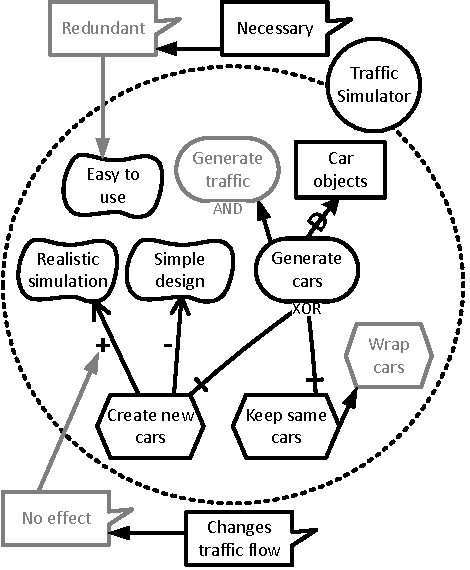
\includegraphics[width=\columnwidth]{img/Example1-new-attack.pdf}
\caption{Example RationalGRL model (extension of Fig.~\ref{fig:example-small})}
\label{fig:example-small3}
\end{figure} 

\begin{definition}[Generic Argument]
\label{def:generic-argument}
A generic argument is a tuple $ga=(id, type, name)$, where:
\begin{itemize}
\item $id\in \mathbb{N}$ is the identifier of the generic argument,
\item $type = GenArg$ states that the tuple is a generic argument,
\item $name\in Names$ is a string description of its name.
\end{itemize}
A set of generic arguments is denoted by $GA$.
\end{definition}

Thus, a generic argument is any element in the RationalGRL model that is not an intentional element or an actor. In the example, some of the generic arguments are $(13, GenArg, \text{Redundant})$ and $(14,$ $GenArg,$ Necessary$)$. Note that a constraint of a GRL model (Definition~\ref{def:grl-model}) is that GRL links should connect IEs, which means that in generic arguments cannot be connected with GRL links. 
 
We can now define \emph{arguments}. 

\begin{definition}[Argument]
\label{def:argument}
An argument $A$ is on of the following tuples:
\begin{itemize}
\item An intentional element $ie$ (Def.~\ref{def:ie}), 
\item An actor $act$ (Def.~\ref{def:actor}),
\item An Actor-IE relation $r_{ActIE}$ (Def.~\ref{def:act-ie-relation}), 
\item A link $link$ (Def.~\ref{def:link}),
\item A generic argument $ga$ (Def.~\ref{def:generic-argument}).
\end{itemize}
\end{definition}

This definition captures the specification in the RationalGRL metamodel (Figure~\ref{fig:metamodel}) in which the class \textsf{Argument} is a superclass of \textsf{GenericArgument} and \textsf{GRLModelElement}. In sum, we define an argument simply as any one of the GRL IEs or links, or a generic argument. 

Examples of arguments in Figure~\ref{fig:example-small3} are $A_5 = (5,$ $Goal,$ Generate cars$, AND)$, $A'_5 = (5, Goal,$ Generate cars$, XOR)$, $A_4 = (4, Softgoal,$ Easy to use) and $A_{13}=(13,$ $ArgElem,$ Redundant$)$. Note that the two arguments $A_5$ and $A'_5$ show an important difference between RationalGRL models and valid GRL models: While a valid GRL model disallows multiple elements with the same identifier (Definition~\ref{def:valid-grl-model}, condition 1), RationalGRL models do not enforce this restriction. This is because it is possible to create multiple arguments for the same element, where each argument contains different content for the same element. However, the set of \emph{accepted} elements in a RationalGRL should all have unique identifier (see Definition~\ref{def:valid-rationalgrl-model}).

\begin{definition}[Attack Link]
\label{def:link:attack}
Given a set of arguments $Arg$, an attack link $att=(A_i,A_j)$ means:
\begin{itemize}
\item $A_i\in Arg$ is the argument performing that attack,
\item $A_j\in Arg$ is the argument being attacked.
\end{itemize}
A set of attack links is denoted by $Att$.
\end{definition}

As an example, take the arguments $A_5$ for the goal `Generate cars' ($AND$ decomposition), $A'_5$ for the goal `Generate cars' ($XOR$ decomposition), $A_4$ for the softgoal `Easy to use' and the generic argument $A_{13}$ (`Redundant') against the softgoal (`Easy to use'). Given these arguments there are two attack links (Figure~\ref{fig:example-small3}), namely $(A'_{5},A_{5})$ and $(A_{13}, A_{4})$.

We now define a RationalGRL model.

\begin{definition}[RationalGRL Model]
\label{def:rationalgrl-model}
A \emph{RationalGRL model} $RatGRL=(Arg, Att)$ consists of a set of arguments $Args$ (Def.~\ref{def:argument}) and a set of attack links $Att$ (Def.~\ref{def:link:attack}).
\end{definition}

The definition of a RationalGRL model collects all the previously defined GRL and RationalGRL elements in a single definition. For completeness, we now provide the full specification of Figure~\ref{fig:example-small3}. Let us first enumerate all the arguments used in this example:

\begin{flalign*}
A_0 = &(0, Actor, \text{Traffic simulator})&\\
A_1 = &(1, Task, \text{Car objects}),&\\
A_2 = &(2, Softgoal, \text{Realistic simulation}),&\\
A_3 = &(3, Softgoal, \text{Simple design}),&\\
A_4 = &(4, Softgoal, \text{Easy to use}),&\\
A_5 = &(5, Goal, \text{Generate cars}, AND),&\\
A'_5 = &(5, Goal, \text{Generate cars}, XOR),&\\
A_6 = &(6, Task, \text{Create new cars}),&\\
A_7 = &(7, Task, \text{Wrap cars}),&\\
A'_7 = &(7, Task, \text{Keep same cars}),&\\
A_8 = &(8, Dep, 4, 1),&\\
A_9 = &(9, PosContr, 6, 2),&\\
A_{10} = &(10, NegContr, 6, 3),&\\
A_{11} = &(11, Decomp, 6, 5),&\\
A_{12} = &(12, Decomp, 7, 5),&\\
A_{13} = &(13, GenArg, \text{Redundant}),&\\
A_{14} = &(14, GenArg, \text{Necessary}),&\\
A_{15} = &(15, GenArg, \text{No effect}),&\\
A_{16} = &(16, GenArg, \text{Changes traffic flow}),&\\
A_{17} = &(ActIE,0,1),\ldots,A_{23}=(ActIE,0,7)&\\
\end{flalign*}
This model is then formalized as $RatGRL=(Arg, Att)$ where:
\begin{flalign*}
Arg = &\{A_0,\ldots,A_5, A'_5,A_6,A_7,A'_7\ldots,A_{23}\}\\
Att= &\{(A'_{5},A_5), (A'_{7},A_{7}), (A_{13},A_{4}), (A_{14},A_{13}),\\
     & (A_{15},A_{9}),(A_{16},A_{15})\}\\
\end{flalign*}

In Figure~\ref{fig:example-small3}, it can be read from that arguments $A_5$, $A_7$, $A_{13}$ and $A_{15}$ are currently disabled (rejected). However, we have not yet make it clear how exactly this is computed. We will do so in the following definitions.
\begin{figure}[b]
\centering
\includegraphics[]{img/Example1-new-arguments.pdf}
\caption{Example argumentation framework, subset of the RationalGRL model from Figure~\ref{fig:example-small3}.}
\label{fig:goalmodeling:arg2}
\end{figure}
In order to compute when an argument is accepted and when it is not we use argumentation semantics.  We use the standard approach by Dung~\cite{Dung1995}. 

\begin{definition}[Argumentation Framework]
\label{def:argumentation-framework}
An \emph{argumentation framework} $AF=(Arg,Att)$ consists of a set of arguments $Arg$ and a set of attack relations $Att\subseteq Arg\times Arg.$
\end{definition}

Note that the definition of a RationalGRL model (Definition~\ref{def:rationalgrl-model}) is exactly the same as the definition for an argumentation framework. This allows us to use the following definitions directly.

\begin{definition}[Attack, conflict-freeness, defense, admissibility, preferred extension] \label{def:semantics}Suppose an argumentation framework $AF=(Arg,Att)$, two sets of arguments $S\cup S'\subseteq Arg$, and some argument $A\in Arg$. We say that
\begin{itemize}
\item $S$ \emph{attacks} $A$ iff some argument in $S$ attacks $A$,
\item $S$ \emph{attacks} $S'$ iff some argument in $S$ attacks some argument in $S'$,
\item $S$ is \emph{conflict-free} iff it does not attack itself,
\item $S$ \emph{defends} $A$ iff for each $B$ such that $B$ attacks $A$, $S$ attacks $B$,
\item $S$ is \emph{admissible} iff $S$ is conflict-free and defends each argument in it.
\item $S$ is a \emph{preferred extension} iff it is a maximal (w.r.t. set inclusion) admissible set.
\end{itemize}
\end{definition}

Let us explain these definitions using the example argumentation framework in Figure~\ref{fig:goalmodeling:arg2}, which is a subset of our RationalGRL model from Figure~\ref{fig:example-small3}, containing only arguments $A_4, A_{5},A'_{5},A_{13}$, and $A_{14}$. In this example, there are five admissible sets: $\{A'_{5}\}$, $\{A_{14}\}$, $\{A'_{5},A_{14}\}$, $\{A_4, A_{14}\}$ and $\{A_4, A'_5, A_{14}\}$. In the admissible sets that contain both $A_{4}$ and $A_{14}$, we say that $A_{14}$ defends $A_4$ against its attacker $A_{13}$. Sets containing both $A_{5}$ and $A'_{5}$, or both $A_{13}$ and either $A_4$ or $A_{14}$ are not conflict free. Sets containing $A_5$ are not admissible, as they do not defend $A_5$. Similarly, sets containing $A_4$ but not $A_{14}$ are not admissible as they do not defend themselves against $A_{13}$. 

The notion of admissible sets gives rise to various possible extensions of an argumentation framework; in this article, we use the preferred extension. In Figure~\ref{fig:goalmodeling:arg2}, there is one preferred extension, namely $\{A_4, A'_5, A_{14}\}$. It is possible to have multiple preferred extensions in cases where the argumentation framework contains cycles. A simple example of such an argumentation framework is shown in Figure~\ref{fig:goalmodeling:arg3}, where arguments $A_x$ and $A_y$ attack each other. There are two preferred extensions, namely $\{A_x\}$ and $\{A_y\}$. Although the algorithms in Section~\ref{sect:algorithms} do not generate mutually attacking arguments such as in Figure~\ref{fig:goalmodeling:arg3}, our formal framework does not explicitly forbid attack cycles in RationalGRL models. We discuss this in more detail in Section~\ref{sect:discussion:futurework}.

\begin{figure}[ht]
\centering
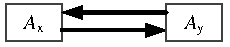
\includegraphics[]{img/example-mutual-attack.pdf}
\caption{Example of a cyclic argumentation framework.}
\label{fig:goalmodeling:arg3}
\end{figure}

The status of individual arguments can now be determined on the basis of the preferred extensions. Recall from the metamodel (Figure~\ref{fig:metamodel}) that an argument can be \emph{acceptable}, \emph{undecided} or \emph{rejected}. 

\begin{definition}[Argument Acceptability] 
\label{def:acceptability}
\begin{itemize}
\item An argument is \emph{acceptable} w.r.t. an argumentation framework $AF$ if it is in every preferred extension of $AF$. 
\item An argument is \emph{undecided} w.r.t. an argumentation framework $AF$ if it is in at least one but not all preferred extensions of $AF$. 
\item An argument is \emph{rejected} w.r.t. an argumentation framework $AF$ if it is in no preferred extension of $AF$. 
\end{itemize}
\end{definition}

Take our two simple examples. In Figure~\ref{fig:goalmodeling:arg2}, we have that arguments $A_4$, $A'_5$ and $A_{14}$ are acceptable and arguments $A_5$ and $A_{13}$ are rejected. In Figure~\ref{fig:goalmodeling:arg3}, both arguments $A_x$ and $A_y$ are undecided. Returning to our larger example from Figure~\ref{fig:example-small3}, we can see that arguments $A_5$, $A_7$, $A_{13}$ and $A_{15}$ are rejected and all the other arguments are acceptable.

\subsection{Translating between RationalGRL and GRL}
\label{sect:formalframework:translation}

Now that we have formalized both a GRL model and a RationalGRL model, we present algorithms to translate between these two models. Both of these two translation algorithms are straightforward, which is result of the fact that the two models are formalized in a very similar way.

\paragraph{GRL to RationalGRL Translation} We start with the translation algorithm from GRL to RationalGRL, which is shown in Algorithm~\ref{alg:translation:to-rationalgrl}. The translation algorithm takes a GRL model $GR=(IE, Act, R_{ActIE}, Link)$ (Definition~\ref{def:grl-model}) as input. On line~\ref{alg:translation:to-rationalgrl:args}, it collects all the elements of the GRL model into a set $Arg$, which represents the set of arguments of the RationalGRL model. On line~\ref{alg:translation:to-rationalgrl:att}, the set of attack links is initialized with an empty set, and the new RationalGRL model $(Arg, Att)$ is returned on line~\ref{alg:translation:to-rationalgrl:return}.

\begin{algorithm}[ht]
  \caption{GRL to RationalGRL Translation}
  \label{alg:translation:to-rationalgrl}
  \begin{algorithmic}[1]
    \Procedure{$ToRationalGRL$}{$GRL$}
    \State $Arg \leftarrow IE\cup Act \cup R_{ActIE}\cup Link$\label{alg:translation:to-rationalgrl:args}
    \State $Att \leftarrow \emptyset$\label{alg:translation:to-rationalgrl:att}
    \State \Return $(Arg, Att)$\label{alg:translation:to-rationalgrl:return}
    \EndProcedure
  \end{algorithmic}
\end{algorithm}

\paragraph{RationalGRL to GRL translation} The translation from a RationalGRL model to a GRL model is given in Algorithm~\ref{alg:translation:to-grl}. First. the arguments are each put in the corresponding GRL component sets. The procedure $ComputeExtensions(Arg,Att)$ (line~\ref{alg:translation:to-grl:extension}) computes the (preferred) extensions of the RationalGRL model (Definition~\ref{def:semantics}). A GRL model is then generated from each of the preferred extensions. This is done by iterating over all arguments in the extension in line~\ref{alg:translation:to-grl:for}. The switch statement on line~\ref{alg:translation:to-grl:switch} then does a case distinction on the type of the arguments -- here, $Arg.type$ refers to the $type$ element in an argument tuple $Arg$ -- and each case ensures the argument is put in the right GRL component. Finally, the algorithm returns a GRL model on line~\ref{alg:translation:to-grl:return}. As an example, compare the RationalGRL model in Figure~\ref{fig:example-small3} to the GRL model in Figure~\ref{fig:example-small}, where the latter is a translation of the former.

\paragraph{Valid RationalGRL model} While we have defined a notion of a \emph{valid GRL model} (Definition~\ref{def:valid-grl-model}), we have not done so for a RationalGRL model yet. We define a RationalGRL model as valid if and only if the RationalGRL to GRL translation results in a valid GRL model. Thus, we do not have to reiterate all conditions on a GRL model, but use the translation algorithm.

\begin{algorithm}[b]
  \caption{RationalGRL to GRL Translation}
  \label{alg:translation:to-grl}
  \begin{algorithmic}[1]
    \Procedure{$ToGRL$}{$RatGRL$}
    \State $Ext \leftarrow ComputeExtensions(Arg,Att)$\label{alg:translation:to-grl:extension}
    \For{$E \in Ext$} 
    \State $IE\leftarrow\emptyset$, $Act\leftarrow\emptyset$, $R_{ActIE}\leftarrow\emptyset$, $Link\leftarrow \emptyset$
    \For{$A\in E$}\label{alg:translation:to-grl:for}
      \Switch{$A.type$}\label{alg:translation:to-grl:switch}
          \Case{$IETypes$}
            \State $IE\leftarrow IE\cup \{A\}$
          \EndCase
          \Case{$Actor$}
            \State $Actor\leftarrow Actor\cup \{A\}$
          \EndCase
          \Case{$ActIE$}
            \State $ActIE\leftarrow ActIE\cup \{A\}$
          \EndCase
          \Case{$LinkTypes$}
            \State $Link\leftarrow Link \cup\{A\}$
          \EndCase
      \EndSwitch
    \EndFor
    \State \Return $(IE,Act,R_{ActIE}, Link)$\label{alg:translation:to-grl:return}
    \EndFor
    \EndProcedure
  \end{algorithmic}
\end{algorithm}

\begin{definition}[Valid RationalGRL Model]
\label{def:valid-rationalgrl-model}
A RationalGRL model $RatGRL = (Arg, Att)$ (Def.~\ref{def:rationalgrl-model})
is a \emph{valid RationalGRL model} iff $ToGRL(RatGRL)$ (Algorithm~\ref{alg:translation:to-grl}) is a valid GRL model (Def.~\ref{def:valid-grl-model}).
\end{definition}


\subsection{Algorithms for argument schemes and critical questions}
\label{sect:algorithms}

We have now formalized a \emph{static} representation of the RationalGRL framework. In this section we formalize algorithms for applying argument schemes and critical questions. These algorithms are applied to RationalGRL models (Definition~\ref{def:rationalgrl-model}) and produce new arguments and attack relations. 

As discussed in Section~\ref{sect:overview}, the argument schemes and critical questions of Table~\ref{table:argument-schemes} all lead to one of three operations: \textsf{INTRO}
introduces a new RationalGRL element and \textsf{DISABLE} creates a new argument that attacks another argument. The \textsf{REPLACE} operation can be seen as a combination of \textsf{INTRO} and \textsf{DISABLE}: a new argument corresponding to a GRL element is added and this new argument attacks a previous version of the element or link. We will discuss all three operations in separate sections below.

In all of the following algorithms, we assume that:
\begin{itemize}
\item The algorithms are applied to some valid RationalGRL model $RatGRL$ (Definition~\ref{def:valid-rationalgrl-model}),
\item The procedure $mintId()$ generates a new unique id.
\end{itemize}

\subsubsection{INTRO algorithms}
\label{sect:formalframework:intro}

The following arguments schemes and critical questions of Table~\ref{table:argument-schemes} fall into this category:
\begin{itemize}
\item AS0-AS12
\item CQ5b, CQ6b, CQ6c, CQ7b, CQ9, CQ10b
\end{itemize}

These type of algorithms are short, and consist simply of adding an argument for the element that is being added. We illustrate this with a single example algorithm for AS5.

\begin{algorithm}[h]
  \caption{AS5: Goal with id $i$ decomposes into task $T$}\label{alg:add-decomp}
  \begin{algorithmic}[1]
    \Procedure{$AS_5$}{$i, T$}
    \State $task\_id\gets mintId()$\label{alg:add-decomp:task-id}
    \State $A_1\leftarrow (task\_id, Task, T)$\label{alg:add-decomp:arg1}
    \State $A_2\leftarrow (mintId(), Decomp, i, task\_id)$\label{alg:add-decomp:arg2}
    \State $Arg\gets Arg\cup \{A_1,A_2\}$\label{alg:add-decomp:add-arg}
    \EndProcedure
  \end{algorithmic}
\end{algorithm}

We have slightly reworded critical question AS5 in Algoritm~\ref{alg:add-decomp}. We assume that a goal $G$ exists already with identifier $i$, and that some new task with name $T$ is a decomposition of $G$. In the algorithm, on line~\ref{alg:add-decomp:task-id} a unique identifier is created for the task, which is created on line~\ref{alg:add-decomp:arg1}. On line~\ref{alg:add-decomp:arg2} an argument is created for the decomposition link $(mintId(), Decomp, i, task\_id)$ (Def.~\ref{def:link}, going from the existing goal with identifier $i$ to the new task with identifier $task\_id$. On line~\ref{alg:add-decomp:add-arg} the two arguments are added to the set of arguments $Arg$.

As an example, suppose we are adding the decomposition of goal ``Generate cars'', expressed as argument $A_5 = (5,$ $Goal,$ Generate cars$, AND)$, into task ``Keep same cars'', and suppose we have the following argument for the goal: . Adding the decomposition can be formalized as executing $AS_5(5, \text{Keep same cars})$, and results in two new arguments: $A_7 = (7, Task, \text{Keep same cars})$ and $A_{12} = (12, Decomp, 7, 5)$, which are both added to the set of arguments $Arg$.

The critical questions of type \emph{INTRO} are all very similar, with one exception: they require an answer. For instance, suppose CQ5b: ``Does goal $G$ decompose into other tasks?'' is answered with: ``Yes, namely into task $T$''. In this case, we simply obtain an instantiation of argument scheme AS5: ``Goal $G$ decomposes into task $T$'', which can be executed with Algorithm~\ref{alg:add-decomp}. This is the same for all the other critical questions of type \emph{INTRO}. Therefore, they are not shown here as well.

\subsubsection{DISABLE algorithms}
\label{sect:formalframework:disable}
As discussed before, algorithms of type \emph{DISABLE} consist of adding a new argument attacking an existing argument. The argument that is added is not an argument for a GRL element or link, but it is rather a generic argument (Definition~\ref{def:generic-argument}).

In the following algorithm, we assume the critical question is answered affirmatively, as indicated in the right-most column of Table~\ref{table:argument-schemes}. For instance, for critical question CQ0 ``Is the actor relevant?'', we assume it is answered with ``No''. In this case, an action is required. In contrary, if the answer to the question is ``Yes'', no action is required.

\begin{algorithm}[h]
  \caption{CQ0: Is actor with id $i$ relevant? No}\label{alg:actor-not-relevant}
  \begin{algorithmic}[1]
    \Procedure{$CQ_0$}{$i$}
    \State $A \leftarrow (mintId(),GenArg,CQ0)$\label{alg:actor-not-relevant:genarg}
    \State $Arg\leftarrow Arg \cup \{A\}$\label{alg:actor-not-relevant:genarg2}
    \For{$A_j\in \{A=(i,Actor,n)\mid A\in Arg\}$}\label{alg:actor-not-relevant:for}
      \State $Att \leftarrow Att \cup \{(A,A_j)\}$\label{alg:actor-not-relevant:att}
    \EndFor
    \EndProcedure
  \end{algorithmic}
\end{algorithm}

Algorithm~\ref{alg:actor-not-relevant} is executed when critical question CQ0 is answered with ``No''. First, on lines~\ref{alg:actor-not-relevant:genarg} and~\ref{alg:actor-not-relevant:genarg2}, an argument is created for the critical question and added to the set of arguments $Arg$. Since this argument is not an argument for a GRL element or link, it is formalized as a \emph{generic counterargument} $(mintId(), GenArg, CQ0)$ (Def.~\ref{def:generic-argument}). The for loop starting at line~\ref{alg:actor-not-relevant:for} then iterates over all arguments for actors, where $i$ is the id of the actor that is no longer relevant. The reason why there could be multiple of such actors is that the actor can be refined by an algorithm of type \emph{REPLACE}. We will explain this in more detail in the example below. Then, on line~\ref{alg:actor-not-relevant:att}, an attack link is created from the generic argument $A$ to the argument for the actor $A_j$. After executing the algorithm, all existing arguments for the actor with identifier $i$ are attacked by a newly created argument $A$.

Consider for example the RationalGRL model in Figures~\ref{fig:examples:relevant-actor}, which consists of an actor and a generic counterargument. Let us reconstruct this model using the application of argument schemes and critical questions to an initially empty RationalGRL model ($Arg=\emptyset$ and $Att=\emptyset$). The algorithm $AS_0(\text{Development team})$ is executed, which results in $A_1=\{(0,Actor,\text{Development team}\})$. After this, critical question CQ0: ``Is the actor Development team relevant?'' is answered with ``No, because the professor develops the software''. We can formalize this as executing algorithm $CQ_0(0)$ (Algorithm~\ref{alg:actor-not-relevant}), which results in adding a generic counter argument $A_2=(1, GenArg, \text{CQ0: Professor develops software})$ and an attack link $(A_2,A_1)$. The RationalGRL model now consists of two arguments, and that the preferred extension is $\{A_2\}$, which means that the resulting GRL model is empty, because generic arguments are not translated to GRL.

Algorithms for the remaining critical questions are omitted here since they are not very complex. 

\begin{figure*}[b]
\centering
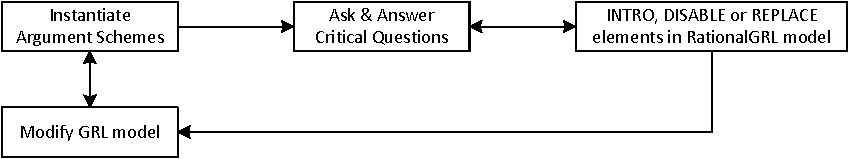
\includegraphics{img/methodology.pdf}
\caption{The RationalGRL Methodology}
\label{fig:rationalgrl-methodology}
\end{figure*}

\subsubsection{REPLACE algorithms}
\label{sect:formalframework:replace}

Recall that \emph{REPLACE} algorithms create a new argument that attacks all arguments for an existing element.

\begin{algorithm}[h]
  \caption{CQ5c: Is the decomposition type of element $ie_i$ correct? No, it should be $X$ }\label{alg:replace1}
  \begin{algorithmic}[1]
    \Procedure{$CQ_{Decomp}$}{$ie_i, X$}
    \State $A \leftarrow ie_i$\label{alg:replace1:arg}
    \State $A.decomptype\leftarrow X$\label{alg:replace1:decompchange}
    \State $IEArgs\leftarrow IE_i\subseteq  Arg$\label{alg:replace1:ieargs}
    \For{$\{(A_i,A_j)\in Att\mid A_j\in IEArgs\}$}\label{alg:replace1:for1}
      \State $Att\leftarrow (A_i,A)$
    \EndFor
    \For{$\{(A_i,A_j)\in Att\mid A_i\in IEArgs\}$}\label{alg:replace1:for2}
      \State $Att\leftarrow (A,A_j)$
    \For{$A_i\in IEArgs$}\label{alg:replace1:for3}
      \State $Att \leftarrow Att \cup \{(A,A_i)\}$\label{alg:replace1:att}
    \EndFor
    \EndFor
    \State $Arg\leftarrow Arg \cup \{A\}$\label{alg:replace1:addarg}
    \EndProcedure
  \end{algorithmic}
\end{algorithm}

While the original critical question CQ5c is specific to the decomposition between a goal and a task, Algorithm~\ref{alg:replace1} is more generally applicable to the decomposition type of any IE, since all IEs have a decomposition type (Definition~\ref{def:ie}). 

Let us go through this algorithm step by step. On line~\ref{alg:replace1:arg}, a new argument $A$ is created which is identical to original IE. On line~\ref{alg:replace1:decompchange} the decomposition type of the argument is changed to $X$ -- here, $Arg.decomptype$ refers to the $decomptype$ element in an argument tuple $Arg$. On line~\ref{alg:replace1:ieargs}, the set $IEArgs$ is assigned with all existing arguments for the input IE -- here $IE_i$ is the set of all IEs with id $i$. The first two for loops on respectively lines~\ref{alg:replace1:for1} and~\ref{alg:replace1:for2} ensure that all attack links that existing from and to the previous versions of the IE are also carried over to the new argument $A$. Then, in the third for loop on line~\ref{alg:replace1:for3}, we add attack links from the argument that has just been created to all existing arguments for the IE. This ensures that all previous version of the IE are not part of the preferred extension, and as a result do not show up in the resulting GRL model. Finally, one line~\ref{alg:replace1:addarg}, the new argument is added to the set of arguments.

As an example, take Figure~\ref{fig:example_AS}. The initial RationalGRL model (before applying CQ10b), can be formalized as follows: $RatGRL=(Arg,Att)$, with $Arg=\{A_1,A_2,A_3,A_4,A_5\}$ and $Att=\emptyset$, where:
\begin{itemize}
\item $A_1=(0,Goal,\text{Simulate traffic},AND)$
\item $A_2=(1,Task,\text{Dynamic simulation},AND)$
\item $A_3=(2,Task,\text{Static simulation},AND)$
\item $A_4=(3,Decomp,1,0)$
\item $A_5=(4,Decomp,2,0)$
\end{itemize}

Suppose algorithm $CQ_{Decomp}(0, XOR)$ is executed for this RationalGRL model. On lines~\ref{alg:replace1:arg} and \ref{alg:replace1:decompchange} a new argument $A_6=(0,Goal,\text{Simulate traffic},OR)$ is created. On line~\ref{alg:replace1:ieargs}, $IEArgs$ contains all arguments for element 0, which is $\{A_1\}$ (note this does not yet include argument $A_6$, since it is not yet added to the RationalGRL model). The first two for loops on lines~\ref{alg:replace1:for1} and~\ref{alg:replace1:for2} do not do anything in the case of our example, since $A_1$ is itself not attack or does not attack any other argument. The for loop on line~\ref{alg:replace1:for3} ensures all previous versions of the element with id 0 are now attacked, which means in our case the $(A_6,A_1)$ is added to $Att$. Finally, on line~\ref{alg:replace1:addarg} the new argument $A_6$ is added to $Arg$.

The other \emph{REPLACE} algorithms are similar to Algorithm~\ref{alg:replace1}, which can be used directly for CQ10c. For CQ12 we should make a small modification: instead of replacing the decomposition type of the IE, we replace its name. Since this is a very minor modification we don't show it here.